\section{Architettura CUDA}

Compute Unified Device Architecture (CUDA) è l'architettura di elaborazione
parallela, basata sul paradigma SIMD,
progettata e sviluppata da NVIDIA che sfrutta la potenza di calcolo delle GPU
per aumentare le prestazioni di alcuni tipi di software.
L'elaborazione sta lentamente migrando verso il paradigma di 
co-processing su CPU e GPU, identificati rispettivamente come
\textit{host} e \textit{device}, il quale prevede che l'esecuzione della
gran parte del carico computazionale venga demandata alla GPU e i risultati
presi nuovamente in carico dalla CPU.
\\
Questo nuovo tipo di paradigma ha trovato immediato seguito nel settore
della ricerca scientifica, dato che ha contribuito in particolare alla nascita
e al miglioramento di software per la simulazione di fenomi fisici e
biologici.

\paragraph{Specifiche Hardware}\mbox{}
\\
Generalmente l'hardware può cambiare con l'avvento di
nuove generazioni di GPU ma la struttura generale si basa sempre sul concetto di
Streaming Multiprocessors (SM) \cite{nickolls2010gpu}

\begin{figure}[H]
    \centering
    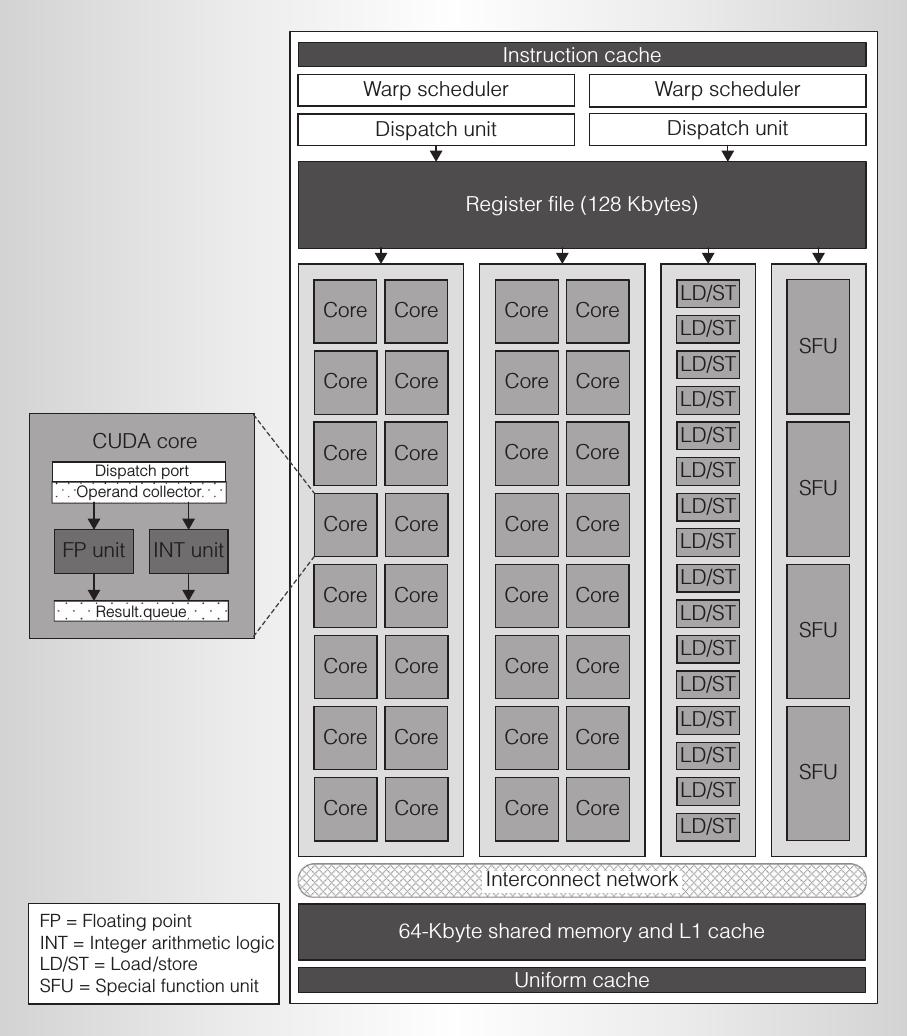
\includegraphics[scale=0.4]{fermi_sm}
    \caption{Streaming Multiprocessor dell'architettura Fermi 
        \cite{nickolls2010gpu}}
    \label{fig:fermi-arch}
\end{figure}

In figura \ref{fig:fermi-arch} è rappresentata schematicamente l'architettura
di uno SM di una GPU NVIDIA della generazione Fermi. Da notare il
numero elevato di core disponibili per l'elaborazione delle istruzioni e la
presenza di due tipi distinti di memorie che risiedono all'interno dello SM:
i registri e la memoria condivisa.

\paragraph{Astrazione Software}\mbox{}
\\
Dato che vengono periodicamente rilasciate nuove versione dell'architettura
hardware delle schede, NVIDIA ha sviluppato delle API per dialogare con la GPU
che sono indipendenti dall'architettura del device utilizzato, rendendo
così possibile lo sviluppo di software portabile su tutte le schede che
supportano CUDA. In generale la maggior parte di queste API è accessibile
attraverso tutte le GPU NVIDIA, altre però richiedono una determinata versione
compute capability ovvero un indicatore che riassume le specifiche
generali del device e le sue caratteristiche, come ad esempio il parallelismo
dinamico che è disponibile solamente su schede con compute capability maggiore
di 3.5.
\\
Il modello astratto definisce tre tipologie di oggetti:

\begin{itemize}
    \item
        thread: singole unità di calcolo, eseguono il codice sorgente;
    \item
        thread block: insieme logico di thread.
        I thread appartenenti
        allo stesso thread block hanno accesso ad un'area di memoria
        condivisa e accessibile solamente da questi ultimi
        (oltre alla memoria globale della GPU).
        È inoltre possibile ottenere la sincronizzazione di tutti i
        thread appartenenti al medesimo thread block;
    \item
        grid: insieme logico di thread block. Non è stata
        prevista un'area di memoria condivisa da tutta la grid
        e fino ad ora non esiste una primitiva per la sincronizzazione fra
        thread block di una specifica grid.
        Per ottenere questo livello di sincronizzazione è necessario
        invocare la primitiva \textit{cudaDeviceSynchronize()}, operazione
        che deve essere effettuata dalla CPU. Essendo una funzione sincrona,
        essa blocca il flusso di esecuzione delle istruzioni della CPU,
        ponendola in stato di attesa rispetto al termine dei kernel
        in esecuzione sulla GPU.
        Risulta quindi buona norma minimizzare l'utilizzo di questa primitiva,
        per evitare rallentamenti significativi all'interno del software.
\end{itemize}

\begin{figure}[H]
    \centering
    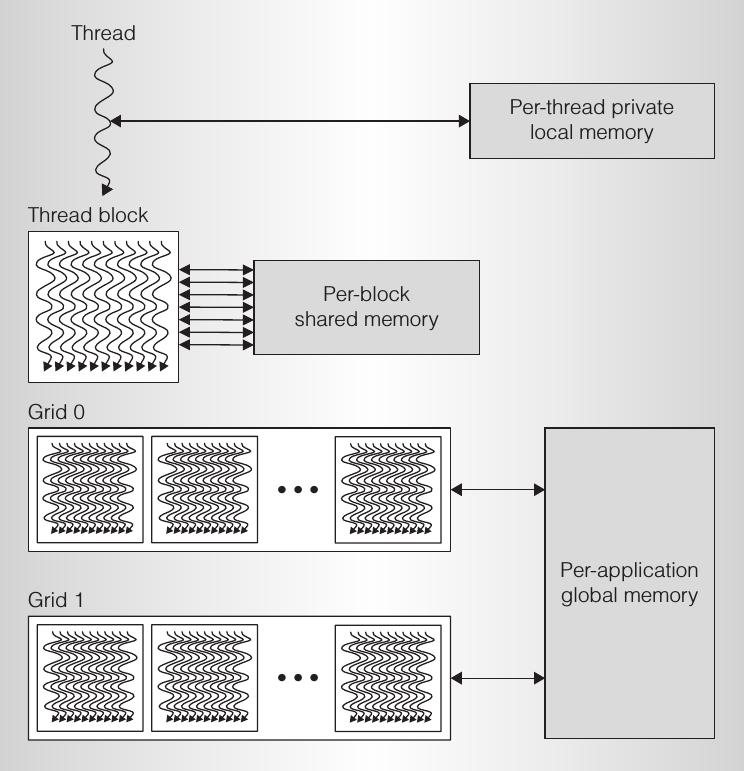
\includegraphics[scale=0.5]{cuda_astraction}
    \caption{Schema della gerarchia di thread, thread block, e grid 
        \cite{nickolls2010gpu}}
\end{figure}

Le procedure che vengono eseguite sulla GPU vengono chiamate kernel
(identificabili grazie al prefisso \textit{\_\_global\_\_})
ed è possibile specificarne la dimensione, ovvero decidere quanti
thread e thread block verranno assegnati
all'esecuzione del codice invocato.
\\
\lstinputlisting[label=kernel, language=C++,
    caption={Esempio di invocazione GPU kernel},
    style=custom]
    {Code/simple_kernel.c}

Come è possibile notare nell'esempio di codice \ref{kernel}, si sta invocando
l'esecuzione di un kernel specificando l'utilizzo di 8 thread block e
32 thread per blocco. In generale il numero totale di
thread che verranno utilizzati per la computazione del kernel è
$$B * T$$ dove $B$ e $T$
sono rispettivamente
il numero di thread block e il numero
di thread per blocco che si vuole utilizzare.

La possibilità di modificare la suddivisione del kernel in thread block
si rivela molto utile nell'elaborazione di strutture dati non
particolarmente complesse, come gli array.
Infatti è sufficiente invocare un kernel con numero di thread
uguale (o maggiore) al numero di elementi dell'array e assegnare la
computazione di ogni elemento ad un singolo e specifico thread.
\\
Esiste però un limite al numero di thread per thread block che è possibile
dichiarare (nelle nuove versioni di CUDA è 1024), dunque per ottenere
l'id globale del thread relativo al kernel eseguito bisogna avvalersi anche
del numero di thread block richiesti durante l'invocazione del kernel,
secondo la seguente relazione:
$$\tau + (\beta * B)$$
dove $B$ e $T$ sono rispettivamente il numero di thread block
e il numero di thread per blocco che
devono essere utilizzati e $\beta$ e $\tau$ sono gli id locali
associati al thread block e
al thread con $\beta < B$ e $\tau < T$.
\\
\lstinputlisting[label=threadid, language=C++,
    caption={Esempio di calcolo dell'id globale associato ad un thread durante
            l'esecuzione di un kernel},
    style=custom]
    {Code/thread_id.c}

\paragraph{Gerarchie di memoria}\mbox{}
\\
Attraverso l'astrazione software CUDA mette a disposizione tre diverse
tipologie di memorie\cite{kirk2007nvidia}:

\begin{itemize}
    \item registri: rappresentano la memoria privata di ogni singolo thread,
        sono estremamente veloci dato che risiedono all'interno del chip.
        Vengono utilizzati per memorizzare le
        variabili locali dichiarate da ogni thread;
    
    \item memoria condivisa: la velocità di accesso è pressochè simile a quella
        dei registri poiché anch'essa è presente all'interno del chip e viene
        suddivisa fra i thread block schedulati sullo Streaming Multiprocessor,
        rendendo possibile lo scambio di informazioni intra blocco evitando
        in alcuni casi l'accesso alla memoria globale quando si tratta di
        utilizzare dati utili solamente all'elaborazione interna al
        blocco stesso.

    \item memoria globale: è il tipo di memoria più lenta poiché non è presente
        direttamente all'interno del chip, ma è un'unità DRAM esterna con grande
        capacità di memorizzazione. Solitamente è utilizzata per le
        comunicazioni inter block e per lo scambio di dati fra CPU e GPU.
\end{itemize}

\paragraph{Gerarchie di esecuzione}\mbox{}
\\
Come descritto in precedenza, un kernel specifica un numero di thread che
andranno ad elaborare i dati, questa operazione si traduce fisicamente
nell'esecuzione dei thread appartenenti a un thread block su uno
Streaming Multiprocessor. All'interno di uno SM possono risiedere
diversi thread block (che non potranno essere migrati su altri SM)
che verranno eseguiti in modo concorrente. Questa scelta è dovuta al fatto
che così facendo è possibile utilizzare la memoria condivisa presente
all'interno di ogni SM, infatti sia il file dei Registri che la Memoria
Condivisa vengono suddivisi equamente fra tutti i thread block in esecuzione
su uno stesso SM, inoltre è disponibile la sincronizzazione fra thread
appartenenti ad un thread block tramite la primitiva \textit{\_\_syncthreads()}.

